\section{The disc-to-strip map and the layer maps}\label{sec:str}

This section constructs the planar disc-to-strip map and proves Proposition~\ref{prop:hdl-strip}. The higher-dimensional layer maps, one ball per layer, are in~\cite{SongHD}.

\medskip\noindent\emph{Conventions.}
On $\C\ni z=x+iy$, $\omega_\C=dx\wedge dy=dI\wedge d\theta$ with $I=\pi|z|^2$, $\theta=\arg z/2\pi$. The strip $(0,\infty)\times(0,1)$ has coordinates $(x,T)$ and area form $dx\wedge dT$. The plane $\R^2\ni\xi=(\xi_1,\xi_2)\cong\C$ ($\xi\mapsto\xi_1+i\xi_2$) carries $d\xi=d\xi_1\wedge d\xi_2$; $\mathrm{Rot}_\phi$ is rotation by $\phi$. In \S\ref{sec:str-balls} (and~\cite{SongHD}) $\C^n=\C\times\C^m\ni(z_{\rm b},z_{\rm f})$, $\varpi=\pi|z_{\rm b}|^2$, $p=p(z_{\rm f})$, so $\omega_0=\omega_\C(z_{\rm b})+\omega_V(z_{\rm f})$, $B(c)=\{\varpi+|p|\le c\}$, $\Bo(c)=\{\varpi+|p|<c\}$.

\subsection{The strip Morse functions}\label{sec:str-morse}

$\Psi_\delta$ sends the circle of area $I$ onto a level set of $R_{\rm st}(x)+V_{\rm st}(T)$ inside $\{x<I+\frac\delta2\}$ (Figure~\ref{fig:str-strip}); it is the product $F_{\rm st}$ of signed square-root inverses $X_{\rm st},Y_{\rm st}$ of $R_{\rm st},V_{\rm st}$, followed by two circle-preserving density normalisations.

\begin{construction}[Strip Morse functions]\label{cons:str-morse}
\lean{SymplecticPacking.Strip.bst, SymplecticPacking.Strip.Rst, SymplecticPacking.Strip.Vst,
SymplecticPacking.Strip.Xst, SymplecticPacking.Strip.Yst, SymplecticPacking.Strip.Jst}
Let $\delta>0$ and $b_{\rm st}=\delta/\pi$. For $x>0$, $0<T<1$ and $\xi=(\xi_1,\xi_2)\in\R^2$ put
\begin{align*}
 R_{\rm st}(x)&=x+\frac{b_{\rm st}^2}{4x}-b_{\rm st}, &
 V_{\rm st}(T)&=b_{\rm st}\Big[\frac{1}{2\sqrt{T(1-T)}}-1\Big],\\
 X_{\rm st}(\xi_1)&=\tfrac12\Big[\xi_1^2+b_{\rm st}+\xi_1\sqrt{\xi_1^2+2b_{\rm st}}\Big], &
 Y_{\rm st}(\xi_2)&=\frac12+\frac{\xi_2\sqrt{\xi_2^2+2b_{\rm st}}}{2(\xi_2^2+b_{\rm st})} ,
\end{align*}
and $F_{\rm st}(\xi)=\big(X_{\rm st}(\xi_1),Y_{\rm st}(\xi_2)\big)$, $\mathcal J_{\rm st}(\xi)=X_{\rm st}'(\xi_1)\,Y_{\rm st}'(\xi_2)$.
\end{construction}

\begin{lemma}[Smooth Morse inverses]\label{lem:str-morse-inverse}
\lean{SymplecticPacking.Strip.Rst_nonneg, SymplecticPacking.Strip.Rst_eq_zero_iff,
 SymplecticPacking.Strip.Vst_nonneg, SymplecticPacking.Strip.Vst_eq_zero_iff,
 SymplecticPacking.Strip.Rst_Xst, SymplecticPacking.Strip.Vst_Yst,
 SymplecticPacking.Strip.deriv_Xst, SymplecticPacking.Strip.deriv_Yst,
 SymplecticPacking.Strip.contDiff_Xst, SymplecticPacking.Strip.contDiff_Yst,
 SymplecticPacking.Strip.Xst_bijOn, SymplecticPacking.Strip.Yst_bijOn}
\uses{cons:str-morse}
\begin{enumerate}[label=(\roman*)]
\item $R_{\rm st}\ge0$ on $(0,\infty)$ with unique zero $x=b_{\rm st}/2$, and $V_{\rm st}\ge0$ on $(0,1)$ with unique zero
$T=\frac12$.
\item $R_{\rm st}(X_{\rm st}(\xi_1))=\xi_1^2$ and $V_{\rm st}(Y_{\rm st}(\xi_2))=\xi_2^2$ for all $\xi_1,\xi_2\in\R$.
\item $X_{\rm st}$ and $Y_{\rm st}$ are smooth on $\R$, with
\[
 X_{\rm st}'(\xi_1)=\frac{\big(\xi_1+\sqrt{\xi_1^2+2b_{\rm st}}\big)^2}{2\sqrt{\xi_1^2+2b_{\rm st}}}>0,\qquad
 Y_{\rm st}'(\xi_2)=\frac{b_{\rm st}^2}{\sqrt{\xi_2^2+2b_{\rm st}}\,(\xi_2^2+b_{\rm st})^2}>0 .
\]
\item $X_{\rm st}$ is an increasing bijection $\R\to(0,\infty)$ and $Y_{\rm st}$ an increasing bijection $\R\to(0,1)$.
$F_{\rm st}$ is a smooth diffeomorphism of $\R^2$ onto $(0,\infty)\times(0,1)$ with
$F_{\rm st}^*(dx\wedge dT)=\mathcal J_{\rm st}\,d\xi$ and $R_{\rm st}\circ X_{\rm st}+V_{\rm st}\circ Y_{\rm st}=|\xi|^2$.
\end{enumerate}
\end{lemma}

\begin{proof}
(i) $R_{\rm st}(x)=(\sqrt x-b_{\rm st}/(2\sqrt x))^2$, which vanishes only at $x=b_{\rm st}/2$. Since $T(1-T)\le\frac14$ with
equality only at $T=\frac12$, $V_{\rm st}\ge0$ with unique zero $T=\frac12$.

(ii) For $x>0$, $R_{\rm st}(x)=\xi_1^2$ is equivalent to $x^2-(\xi_1^2+b_{\rm st})x+b_{\rm st}^2/4=0$, with discriminant
$(\xi_1^2+b_{\rm st})^2-b_{\rm st}^2=\xi_1^2(\xi_1^2+2b_{\rm st})$ and roots
$x_\pm=\frac12[\xi_1^2+b_{\rm st}\pm|\xi_1|\sqrt{\xi_1^2+2b_{\rm st}}]$, both positive because $x_+x_-=b_{\rm st}^2/4$.
$X_{\rm st}(\xi_1)$ is $x_+$ for $\xi_1\ge0$ and $x_-$ for $\xi_1\le0$. For the second identity write $Y_{\rm st}=\frac12+\tau$
with $\tau=\xi_2\sqrt{\xi_2^2+2b_{\rm st}}/(2(\xi_2^2+b_{\rm st}))$. Then
$\tau^2=\frac14-\frac{b_{\rm st}^2}{4(\xi_2^2+b_{\rm st})^2}<\frac14$, so $0<Y_{\rm st}<1$,
$T(1-T)=\frac14-\tau^2=b_{\rm st}^2/(4(\xi_2^2+b_{\rm st})^2)$ for $T=Y_{\rm st}(\xi_2)$, hence
$1/(2\sqrt{T(1-T)})=(\xi_2^2+b_{\rm st})/b_{\rm st}$ and $V_{\rm st}(T)=\xi_2^2$.

(iii) Smoothness holds because $\xi_1^2+2b_{\rm st}>0$ and $\xi_2^2+b_{\rm st}>0$. With $r=\sqrt{\xi_1^2+2b_{\rm st}}$,
$2X_{\rm st}'=2\xi_1+r+\xi_1^2/r=(\xi_1+r)^2/r$, and $\xi_1+r>0$ since $r>|\xi_1|$. With
$\varphi(\xi_2)=\xi_2\sqrt{\xi_2^2+2b_{\rm st}}/(\xi_2^2+b_{\rm st})$,
\[
 \varphi'(\xi_2)=\frac{(2\xi_2^2+2b_{\rm st})(\xi_2^2+b_{\rm st})-2\xi_2^2(\xi_2^2+2b_{\rm st})}
 {\sqrt{\xi_2^2+2b_{\rm st}}\,(\xi_2^2+b_{\rm st})^2}
 =\frac{2b_{\rm st}^2}{\sqrt{\xi_2^2+2b_{\rm st}}\,(\xi_2^2+b_{\rm st})^2},
\]
and $Y_{\rm st}'=\varphi'/2$.

(iv) Both maps are continuous and strictly increasing by (iii). As $\xi_1\to+\infty$, $X_{\rm st}\to\infty$; for $\xi_1<0$,
$X_{\rm st}(\xi_1)=x_-=b_{\rm st}^2/(4x_+)$ with $x_+\to\infty$ as $\xi_1\to-\infty$, so $X_{\rm st}\to0^+$. Since $\varphi$ is odd
and $\varphi^2=1-b_{\rm st}^2/(\xi_2^2+b_{\rm st})^2\to1$, $Y_{\rm st}$ increases from $0^+$ to $1^-$. Thus $F_{\rm st}$ is a
smooth bijection with Jacobian $\mathcal J_{\rm st}>0$, hence a smooth diffeomorphism by the inverse function theorem;
the last identity is (ii).
\end{proof}

\subsection{The strip map}\label{sec:str-map}

The two normalisations are those of Definition~\ref{def:pln-normalisations} for one density, in Cartesian coordinates; we repeat the proofs since $\mathcal J_{\rm st}$ is not constant near the origin, as setting (N) of \S\ref{sec:pln-normalisation-maps} assumes.

\begin{definition}[Rotation and area normalisation]\label{def:str-normalisation}
\lean{SymplecticPacking.Inner.Jbar, SymplecticPacking.Inner.Bfun, SymplecticPacking.Inner.Trot,
 SymplecticPacking.Inner.Acal, SymplecticPacking.Inner.Acal_strictMono, SymplecticPacking.Inner.Acal_bijective,
 SymplecticPacking.Inner.Einv, SymplecticPacking.Inner.Darea}
Let $\mathcal J$ be a positive smooth function on $\R^2$. Put
\begin{align*}
 \bar{\mathcal J}(|\xi|^2)&=\frac1{2\pi}\int_0^{2\pi}\mathcal J(\mathrm{Rot}_\phi\xi)\,d\phi,\\
 \mathcal M(\xi)&=\frac1{2\pi}\int_0^{2\pi}(\phi-\pi)\,\mathcal J(\mathrm{Rot}_\phi\xi)\,d\phi,\\
 \mathsf T_{\mathcal J}(\xi)&=\mathrm{Rot}_{\mathcal M(\xi)/\bar{\mathcal J}(|\xi|^2)}\,\xi .
\end{align*}
and $\mathfrak a_{\mathcal J}(\mathcal E)=\int_{|\xi|^2\le\mathcal E}\mathcal J\,d\xi$ for $\mathcal E\ge0$. In polar coordinates
$\mathfrak a_{\mathcal J}(\mathcal E)=\int_0^{\sqrt{\mathcal E}}\int_0^{2\pi}\mathcal J\,d\psi\,r\,dr
=\int_0^{\sqrt{\mathcal E}}2\pi r\bar{\mathcal J}(r^2)\,dr=\pi\int_0^{\mathcal E}\bar{\mathcal J}(t)\,dt$ with $\bar{\mathcal J}>0$, so
$\mathfrak a_{\mathcal J}$ is continuous and strictly increasing with $\mathfrak a_{\mathcal J}(0)=0$. If
$\mathfrak a_{\mathcal J}(\mathcal E)\to\infty$ as $\mathcal E\to\infty$, it is a bijection of $[0,\infty)$; then let
$\mathcal E_{\mathcal J}=\mathfrak a_{\mathcal J}^{-1}$ and, for $z\in\C$ with $I=\pi|z|^2$,
\[
 \mathsf D_{\mathcal J}(z)=\sqrt{\pi\,\mathcal E_{\mathcal J}(I)/I}\;z\quad(z\ne0),\qquad \mathsf D_{\mathcal J}(0)=0 .
\]
\end{definition}

\begin{lemma}[Normalisation]\label{lem:str-normalisation}
\lean{SymplecticPacking.Inner.Trot_bijective, SymplecticPacking.Inner.Trot_det,
 SymplecticPacking.Inner.Darea_bijective, SymplecticPacking.Inner.norm_Darea_sq,
 SymplecticPacking.Inner.Darea_pullback, SymplecticPacking.Strip.normalize_general}
\uses{def:str-normalisation}
Let $\mathcal J$ be a positive smooth function on $\R^2$.
\begin{enumerate}[label=(\roman*)]
\item $\mathsf T_{\mathcal J}$ is a smooth diffeomorphism of $\R^2$ which maps every circle
$\{|\xi|=r\}$ onto itself, and $\mathsf T_{\mathcal J}^*\big(\bar{\mathcal J}(|\xi|^2)\,d\xi\big)=\mathcal J\,d\xi$.
\item If $\mathfrak a_{\mathcal J}(\mathcal E)\to\infty$, then $\mathsf D_{\mathcal J}$ is a smooth
diffeomorphism $\C\to\R^2$ with $|\mathsf D_{\mathcal J}(z)|^2=\mathcal E_{\mathcal J}(\pi|z|^2)$ and
$\mathsf D_{\mathcal J}^*\big(\bar{\mathcal J}(|\xi|^2)\,d\xi\big)=\omega_\C$.
\item If $\mathfrak a_{\mathcal J}(\mathcal E)\to\infty$ and $F\colon\R^2\to U$ is a smooth
diffeomorphism onto an open set $U\subset\R^2$ with $F^*(dx\wedge dT)=\mathcal J\,d\xi$, then
$F\circ\mathsf T_{\mathcal J}^{-1}\circ\mathsf D_{\mathcal J}\colon\C\to U$ is a smooth
diffeomorphism which pulls $dx\wedge dT$ back to $\omega_\C$ and maps the circle $\{\pi|z|^2=I\}$ onto
$F(\{|\xi|^2=\mathcal E_{\mathcal J}(I)\})$.
\end{enumerate}
\end{lemma}

\begin{proof}
Differentiating under the integral, $\mathcal M$ and $\bar{\mathcal J}(|\xi|^2)>0$ are smooth; bijections with nonvanishing Jacobian are diffeomorphisms.

(i) Fix $r>0$, $\mathcal J_r(\psi)=\mathcal J(re^{i\psi})$. Integrating by parts in $\mathcal M(re^{i\psi})=\frac1{2\pi}\int_0^{2\pi}(\phi-\pi)\mathcal J_r(\psi+\phi)\,d\phi$ gives $\partial_\psi\mathcal M=\mathcal J_r(\psi)-\bar{\mathcal J}(r^2)$. So $\mathsf T_{\mathcal J}(re^{i\psi})=re^{i\Theta(\psi)}$ with $\Theta'=\mathcal J/\bar{\mathcal J}>0$, $\Theta(\psi+2\pi)=\Theta(\psi)+2\pi$; hence $\mathsf T_{\mathcal J}$ is a smooth bijection preserving each circle, and off $0$, $\mathsf T_{\mathcal J}^*(\bar{\mathcal J}\,r\,dr\wedge d\psi)=\bar{\mathcal J}\,r\,dr\wedge(\partial_r\Theta\,dr+\Theta'\,d\psi)=\mathcal J\,r\,dr\wedge d\psi$. Thus $\det D\mathsf T_{\mathcal J}=\mathcal J/\bar{\mathcal J}>0$, also at $0$ by continuity.

(ii) $G(\xi)=\int_0^1\bar{\mathcal J}(t|\xi|^2)\,dt=\frac1{2\pi}\int_0^1\!\int_0^{2\pi}2r\,\mathcal J(\mathrm{Rot}_\phi(r\xi))\,d\phi\,dr$ is smooth, positive, and $\pi|\xi|^2G(\xi)=\mathfrak a_{\mathcal J}(|\xi|^2)$. Hence $\mathsf D'(\xi)=\sqrt{G(\xi)}\,\xi$ preserves the argument, satisfies $\pi|\mathsf D'(\xi)|^2=\mathfrak a_{\mathcal J}(|\xi|^2)$, is a bijection, and inverts $\mathsf D_{\mathcal J}$. With $\mathcal E=|\xi|^2$, off $0$, $(\mathsf D')^*\omega_\C=(\mathsf D')^*(dI\wedge d\psi/2\pi)=\tfrac12\bar{\mathcal J}(\mathcal E)\,d\mathcal E\wedge d\psi=\bar{\mathcal J}\,d\xi$, so $\det D\mathsf D'=\bar{\mathcal J}>0$ (also at $0$). Thus $\mathsf D_{\mathcal J}=(\mathsf D')^{-1}$ is a diffeomorphism with $\mathsf D_{\mathcal J}^*(\bar{\mathcal J}\,d\xi)=\omega_\C$, and $|\mathsf D_{\mathcal J}(z)|^2=\mathcal E_{\mathcal J}(I)$.

(iii) By (i),(ii) the composite is a diffeomorphism onto $U$ with pullback $\mathsf D_{\mathcal J}^*(\mathsf T_{\mathcal J}^{-1})^*(\mathcal J\,d\xi)=\mathsf D_{\mathcal J}^*(\bar{\mathcal J}\,d\xi)=\omega_\C$; $\mathsf D_{\mathcal J}$ maps $\{\pi|z|^2=I\}$ onto $\{|\xi|^2=\mathcal E_{\mathcal J}(I)\}$, preserved by $\mathsf T_{\mathcal J}^{-1}$.
\end{proof}

For $\mathcal J=\mathcal J_{\rm st}$ write $\bar{\mathcal J}_{\rm st}$ and $\mathfrak a_{\rm st}=\mathfrak a_{\mathcal J_{\rm st}}$.

\begin{lemma}[Sublevel sets and area]\label{lem:str-area}
\lean{SymplecticPacking.Strip.width_sublevel, SymplecticPacking.Strip.lt_of_Rst_le,
 SymplecticPacking.Strip.sublevel_empty, SymplecticPacking.Strip.integral_Vst,
 SymplecticPacking.Strip.Ast_eq_integral, SymplecticPacking.Strip.Fst_bijOn, SymplecticPacking.Strip.Fst_det, SymplecticPacking.Strip.level_Fst, SymplecticPacking.Strip.Ast_ge,
 SymplecticPacking.Strip.Ast_Est, SymplecticPacking.Strip.gAcal_strictMono, SymplecticPacking.Strip.gAcal_zero, SymplecticPacking.Strip.Ast_tendsto, SymplecticPacking.Strip.gAcal_hasDerivAt}
\uses{cons:str-morse, lem:str-morse-inverse, def:str-normalisation}
Let $b_{\rm st}=\delta/\pi$.
\begin{enumerate}[label=(\roman*)]
\item For $c\ge0$, $\{x>0:R_{\rm st}(x)\le c\}=[x_-(c),x_+(c)]$ with
$x_\pm(c)=\frac12\big[c+b_{\rm st}\pm\sqrt{c(c+2b_{\rm st})}\big]$. Its length is $\sqrt{c(c+2b_{\rm st})}\ge c$, and
$0<x_-(c)\le x_+(c)<c+b_{\rm st}$. For $c<0$ the set is empty.
\item $\int_0^1V_{\rm st}(T)\,dT=b_{\rm st}(\frac\pi2-1)$.
\item $\mathfrak a_{\rm st}(\mathcal E)$ is the $dx\,dT$-area of $\{(x,T):R_{\rm st}(x)+V_{\rm st}(T)\le\mathcal E\}$, and
$\mathfrak a_{\rm st}(\mathcal E)\ge\mathcal E-b_{\rm st}(\frac\pi2-1)$.
\item $\mathfrak a_{\rm st}$ is a continuous strictly increasing bijection of $[0,\infty)$, with
$\mathfrak a_{\rm st}'(\mathcal E)=\pi\bar{\mathcal J}_{\rm st}(\mathcal E)>0$.
\end{enumerate}
\end{lemma}

\begin{proof}
(i) As in Lemma~\ref{lem:str-morse-inverse}(ii) with $\xi_1^2=c$; $x_+-x_-=\sqrt{c(c+2b_{\rm st})}\ge c$, and $(c+b_{\rm st})^2-c(c+2b_{\rm st})=b_{\rm st}^2>0$ gives $x_->0$, $x_+<c+b_{\rm st}$. For $c<0$ use $R_{\rm st}\ge0$.
(ii) $T=\sin^2\phi$ gives $\int_0^1dT/\sqrt{T(1-T)}=\pi$.
(iii) The first claim is change of variables via $F_{\rm st}$ (Lemma~\ref{lem:str-morse-inverse}(iv)). By Fubini, (i), (ii): $\mathfrak a_{\rm st}(\mathcal E)=\int_0^1|\{x>0:R_{\rm st}(x)\le\mathcal E-V_{\rm st}(T)\}|\,dT\ge\int_0^1(\mathcal E-V_{\rm st})_+\,dT\ge\mathcal E-b_{\rm st}(\tfrac\pi2-1)$.
(iv) From $\mathfrak a_{\rm st}=\pi\int_0^{\mathcal E}\bar{\mathcal J}_{\rm st}$ (Definition~\ref{def:str-normalisation}) and (iii) for $\mathfrak a_{\rm st}\to\infty$.
\end{proof}

\begin{construction}[The strip map]\label{cons:str-map}
\lean{SymplecticPacking.Strip.Ast, SymplecticPacking.Strip.psiStrip}
\uses{cons:str-morse, lem:str-morse-inverse, def:str-normalisation, lem:str-area}
For $\delta>0$ let $\mathsf T_{\rm st}=\mathsf T_{\mathcal J_{\rm st}}$, $\mathcal E_{\rm st}=\mathfrak a_{\rm st}^{-1}$ (defined on
$[0,\infty)$ by Lemma~\ref{lem:str-area}(iv)) and $\mathsf D_{\rm st}=\mathsf D_{\mathcal J_{\rm st}}$, and define
\[
 \Psi_\delta=F_{\rm st}\circ\mathsf T_{\rm st}^{-1}\circ\mathsf D_{\rm st}\colon\C\to(0,\infty)\times(0,1),\qquad
 \Psi_\delta(z)=(x,T).
\]
\end{construction}

\begin{proposition}[Disc-to-strip map]\label{prop:str-strip}
\lean{SymplecticPacking.Strip.psiStrip_smooth, SymplecticPacking.Strip.psiStrip_symplectic,
 SymplecticPacking.Strip.psiStrip_level, SymplecticPacking.Strip.psiStrip_bijOn,
 SymplecticPacking.Strip.psiStrip_x_pos, SymplecticPacking.Strip.psiStrip_x_lt,
 SymplecticPacking.Strip.psiStrip_mem, SymplecticPacking.Strip.x_lower_margin,
 SymplecticPacking.Strip.T_margin}
\uses{cons:str-map, lem:str-normalisation, lem:str-area, lem:str-morse-inverse}
Let $\delta>0$ and $b_{\rm st}=\delta/\pi$. Then:
\begin{enumerate}[label=(\roman*)]
\item $\Psi_\delta$ is a smooth diffeomorphism of $\C$ onto $(0,\infty)\times(0,1)$ with
$\Psi_\delta^*(dx\wedge dT)=\omega_\C$;
\item $R_{\rm st}(x)+V_{\rm st}(T)=\mathcal E_{\rm st}(\pi|z|^2)$ for $(x,T)=\Psi_\delta(z)$;
\item for every $z\in\C$, with $(x,T)=\Psi_\delta(z)$,
\begin{equation}\label{eq:str-x-bound}
 0<x<\pi|z|^2+\frac\delta2,\qquad 0<T<1;
\end{equation}
\item for $I_{\max}\ge0$, $\mathcal E_{\max}=I_{\max}+b_{\rm st}(\frac\pi2-1)$ and $\pi|z|^2\le I_{\max}$,
\[
 x\ge\tfrac12\Big[\mathcal E_{\max}+b_{\rm st}-\sqrt{\mathcal E_{\max}(\mathcal E_{\max}+2b_{\rm st})}\Big]>0,\qquad
 \big|T-\tfrac12\big|\le\tfrac12\sqrt{1-(1+\mathcal E_{\max}/b_{\rm st})^{-2}}<\tfrac12 .
\]
\end{enumerate}
In particular $\Psi_\delta$ has the properties stated in Proposition~\ref{prop:hdl-strip}.
\end{proposition}

\begin{figure}[ht]
\centering
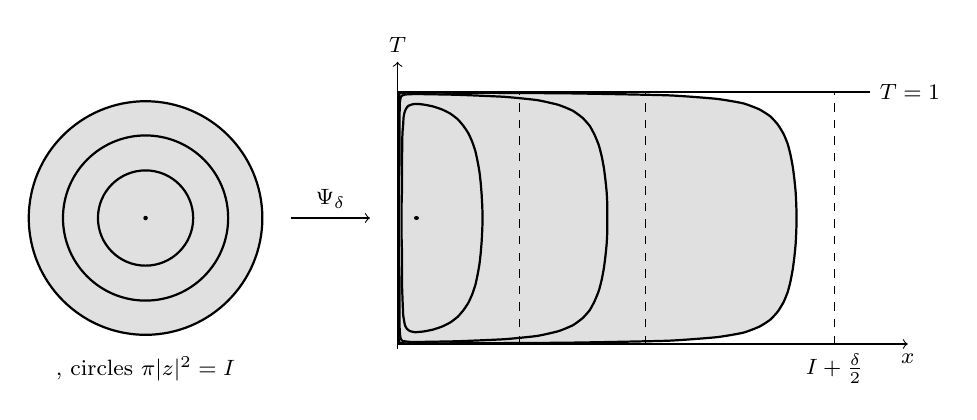
\begin{tikzpicture}[font=\footnotesize]
 \begin{scope}[scale=2.4]
  \fill[black!12] (0,0) circle (0.618);
  \draw[thick] (0,0) circle (0.252);
  \draw[thick] (0,0) circle (0.437);
  \draw[thick] (0,0) circle (0.618);
  \fill (0,0) circle (0.012);
  \node at (0,-0.8) {$\C$, circles $\pi|z|^2=I$};
 \end{scope}
 \draw[->] (1.85,0) -- node[above] {$\Psi_\delta$} (2.85,0);
 \begin{scope}[shift={(3.2,-1.6)},x=4cm,y=3.2cm]
  \fill[black!12] plot[smooth cycle,tension=0.3] coordinates {(0.060,0.002) (0.529,0.005) (0.858,0.013) (1.013,0.027) (1.098,0.045) (1.149,0.069) (1.184,0.097) (1.208,0.130) (1.226,0.167) (1.239,0.207) (1.248,0.251) (1.255,0.298) (1.260,0.346) (1.264,0.397) (1.266,0.448) (1.267,0.500) (1.266,0.552) (1.264,0.603) (1.260,0.654) (1.255,0.702) (1.248,0.749) (1.239,0.793) (1.226,0.833) (1.208,0.870) (1.184,0.903) (1.149,0.931) (1.098,0.955) (1.013,0.973) (0.858,0.987) (0.529,0.995) (0.060,0.998) (0.009,0.996) (0.005,0.989) (0.004,0.977) (0.003,0.960) (0.003,0.937) (0.003,0.910) (0.003,0.879) (0.003,0.843) (0.003,0.803) (0.003,0.760) (0.003,0.714) (0.003,0.666) (0.003,0.616) (0.003,0.565) (0.003,0.513) (0.003,0.461) (0.003,0.409) (0.003,0.359) (0.003,0.310) (0.003,0.262) (0.003,0.218) (0.003,0.177) (0.003,0.139) (0.003,0.105) (0.003,0.076) (0.003,0.051) (0.003,0.031) (0.004,0.016) (0.006,0.006) (0.026,0.002)};
  \draw[thick] plot[smooth cycle,tension=0.3] coordinates {(0.060,0.047) (0.084,0.050) (0.112,0.057) (0.141,0.069) (0.168,0.086) (0.191,0.108) (0.209,0.134) (0.225,0.164) (0.237,0.197) (0.247,0.234) (0.254,0.274) (0.260,0.316) (0.264,0.360) (0.267,0.406) (0.269,0.453) (0.270,0.500) (0.269,0.547) (0.267,0.594) (0.264,0.640) (0.260,0.684) (0.254,0.726) (0.247,0.766) (0.237,0.803) (0.225,0.836) (0.209,0.866) (0.191,0.892) (0.168,0.914) (0.141,0.931) (0.112,0.943) (0.084,0.950) (0.060,0.953) (0.047,0.951) (0.034,0.945) (0.027,0.934) (0.022,0.918) (0.019,0.898) (0.018,0.873) (0.016,0.844) (0.015,0.812) (0.015,0.776) (0.014,0.737) (0.014,0.695) (0.014,0.651) (0.014,0.606) (0.013,0.559) (0.013,0.512) (0.013,0.464) (0.013,0.417) (0.014,0.371) (0.014,0.327) (0.014,0.284) (0.014,0.244) (0.015,0.206) (0.016,0.172) (0.017,0.141) (0.018,0.114) (0.021,0.091) (0.024,0.073) (0.030,0.060) (0.040,0.051) (0.055,0.047)};
  \draw[dashed] (0.388,0) -- (0.388,1);
  \draw[thick] plot[smooth cycle,tension=0.3] coordinates {(0.060,0.008) (0.191,0.011) (0.339,0.019) (0.443,0.032) (0.511,0.051) (0.556,0.074) (0.587,0.102) (0.610,0.134) (0.626,0.171) (0.639,0.211) (0.648,0.254) (0.655,0.300) (0.660,0.348) (0.664,0.398) (0.666,0.449) (0.666,0.500) (0.666,0.551) (0.664,0.602) (0.660,0.652) (0.655,0.700) (0.648,0.746) (0.639,0.789) (0.626,0.829) (0.610,0.866) (0.587,0.898) (0.556,0.926) (0.511,0.949) (0.443,0.968) (0.339,0.981) (0.191,0.989) (0.060,0.992) (0.024,0.990) (0.012,0.984) (0.009,0.972) (0.007,0.955) (0.007,0.932) (0.006,0.905) (0.006,0.874) (0.006,0.839) (0.006,0.799) (0.006,0.757) (0.006,0.712) (0.005,0.664) (0.005,0.615) (0.005,0.564) (0.005,0.513) (0.005,0.461) (0.005,0.410) (0.005,0.360) (0.005,0.312) (0.006,0.265) (0.006,0.221) (0.006,0.181) (0.006,0.143) (0.006,0.110) (0.006,0.081) (0.007,0.056) (0.008,0.036) (0.010,0.022) (0.016,0.012) (0.043,0.008)};
  \draw[dashed] (0.788,0) -- (0.788,1);
  \draw[thick] plot[smooth cycle,tension=0.3] coordinates {(0.060,0.002) (0.529,0.005) (0.858,0.013) (1.013,0.027) (1.098,0.045) (1.149,0.069) (1.184,0.097) (1.208,0.130) (1.226,0.167) (1.239,0.207) (1.248,0.251) (1.255,0.298) (1.260,0.346) (1.264,0.397) (1.266,0.448) (1.267,0.500) (1.266,0.552) (1.264,0.603) (1.260,0.654) (1.255,0.702) (1.248,0.749) (1.239,0.793) (1.226,0.833) (1.208,0.870) (1.184,0.903) (1.149,0.931) (1.098,0.955) (1.013,0.973) (0.858,0.987) (0.529,0.995) (0.060,0.998) (0.009,0.996) (0.005,0.989) (0.004,0.977) (0.003,0.960) (0.003,0.937) (0.003,0.910) (0.003,0.879) (0.003,0.843) (0.003,0.803) (0.003,0.760) (0.003,0.714) (0.003,0.666) (0.003,0.616) (0.003,0.565) (0.003,0.513) (0.003,0.461) (0.003,0.409) (0.003,0.359) (0.003,0.310) (0.003,0.262) (0.003,0.218) (0.003,0.177) (0.003,0.139) (0.003,0.105) (0.003,0.076) (0.003,0.051) (0.003,0.031) (0.004,0.016) (0.006,0.006) (0.026,0.002)};
  \draw[dashed] (1.388,0) -- (1.388,1);
  \draw (0,0) -- (1.5,0);
  \draw (0,1) -- (1.5,1) node[right] {$T=1$};
  \draw[->] (0,-0.02) -- (0,1.12) node[above] {$T$};
  \draw[->] (0,0) -- (1.62,0) node[below] {$x$};
  \fill (0.06,0.5) circle (0.008);
  \node[below] at (1.388,0) {$I+\frac\delta2$};
 \end{scope}
\end{tikzpicture}
\caption{The disc-to-strip map $\Psi_\delta$ of Proposition~\ref{prop:str-strip}: computed level sets for $b_{\rm st}=\delta/\pi=0.12$
and $I=0.2,\,0.6,\,1.2$. The circle of area $I$ goes to the level set $\{R_{\rm st}+V_{\rm st}=\mathcal E_{\rm st}(I)\}$, of
area $I$, inside $\{x<I+\frac\delta2\}$ (dashed); the dot is the common minimum $(b_{\rm st}/2,\frac12)$. Axes not to the same scale.}
\label{fig:str-strip}
\end{figure}

\begin{proof}
(i), (ii) Lemma~\ref{lem:str-normalisation}(iii) applied to $\mathcal J_{\rm st}$ and $F_{\rm st}$ (Lemma~\ref{lem:str-morse-inverse}(iv)), with $\mathfrak a_{\rm st}\to\infty$ by Lemma~\ref{lem:str-area}(iii); the level identity follows from $R_{\rm st}\circ X_{\rm st}+V_{\rm st}\circ Y_{\rm st}=|\xi|^2$.
(iii) Let $I=\pi|z|^2$, $\mathcal E=\mathcal E_{\rm st}(I)$; by Lemma~\ref{lem:str-area}(iii), $I\ge\mathcal E-b_{\rm st}(\frac\pi2-1)$. By (ii) and $V_{\rm st}\ge0$, $R_{\rm st}(x)\le\mathcal E$, so Lemma~\ref{lem:str-area}(i) gives $x<\mathcal E+b_{\rm st}\le I+b_{\rm st}\tfrac\pi2=I+\tfrac\delta2$; the remaining bounds hold since $\Psi_\delta$ maps into the strip.
(iv) Since $\mathcal E_{\rm st}$ increases and $I_{\max}\ge\mathcal E_{\rm st}(I_{\max})-b_{\rm st}(\frac\pi2-1)$ (Lemma~\ref{lem:str-area}(iii)), $\mathcal E=\mathcal E_{\rm st}(\pi|z|^2)\le\mathcal E_{\max}$. By (ii), $R_{\rm st}(x)\le\mathcal E_{\max}$, so $x\ge x_-(\mathcal E_{\max})>0$ (Lemma~\ref{lem:str-area}(i)); and $V_{\rm st}(T)\le\mathcal E_{\max}$, i.e.\ $2\sqrt{T(1-T)}\ge(1+\mathcal E_{\max}/b_{\rm st})^{-1}$, equivalently $(T-\frac12)^2=\frac14-T(1-T)\le\frac14[1-(1+\mathcal E_{\max}/b_{\rm st})^{-2}]$.
\end{proof}

\subsection{Enlarged capacities}\label{sec:str-balls}

The higher-dimensional layer maps of~\cite{SongHD} and the four-dimensional ones of \S\ref{sec:shd-four} use the
following capacities between $\rho_i$ and the auxiliary capacities $a_i$.

\begin{definition}[Enlarged capacities]\label{def:str-enlarged}
\lean{SymplecticPacking.HighDim.RawToricModel.packingSource,
SymplecticPacking.Branch2.CubicData.rhoBar, SymplecticPacking.Branch2.CubicData.deltaStrip,
SymplecticPacking.Branch2.CubicData.rhoHat}
For $1\le i\le k$ put
\[
 \delta_i=\frac{a_i-\rho_i}2,\qquad
 \bar\rho_i=a_i-\frac34\delta_i,\qquad \hat\rho_i=a_i-\frac{\delta_i}2 .
\]
($\bar\rho_i$: closed enlarged source capacity; $\hat\rho_i$: open domain capacity.) Then
$\rho_i<\frac{\rho_i+a_i}2=a_i-\delta_i<\bar\rho_i<\hat\rho_i<a_i$. Put
$\varepsilon_i=(a_i-\hat\rho_i)/4=\delta_i/8$; the $i$-th ball is placed by $\Psi_{\varepsilon_i}$.
In the four-dimensional branch (\S\ref{sec:shd-four}) the same letters denote different values:
there $\bar\rho_i=(\rho_i+a_i)/2=a_i-\delta_i$, $\hat\rho_i=a_i-\frac34\delta_i$, and the $i$-th ball is placed by
$\Psi_{\delta_i}$ (Proposition~\ref{prop:shd4-maps}). The two branches never occur together.
\end{definition}
